\documentclass[a4paper]{article}

\usepackage[english]{babel}
\usepackage[latin1]{inputenc}
\usepackage{amssymb}
\usepackage{framed}
\usepackage{graphicx}
\usepackage{subcaption}
\usepackage{float}

\setlength{\parindent}{0pt}
\setlength{\parskip}{3ex}

\begin{document}

\begin{center}
  {\large Artificial Neural Networks and Deep Architectures, DD2437}\\
  \vspace{7mm}
  {\huge Short report on lab assignment 4\\[1ex]}
  {\Large Restricted Boltzmann Machines and Deep Belief Nets}\\
  \vspace{8mm}
  {\Large Etienne Jodry, Frano Rajic, Ivan Stresec\\}
  \vspace{4mm}
  {\large October 9, 2020\\}
\end{center}

\section{Main objectives and scope of the assignment}

Our major goals in the assignment were:
\begin{itemize}
    \item Gain insight into implementation details of RBMs and DBNs
    \item Applying basic algorithms for unsupervised greedy pre-training of RBM layers
    \item Analyze the abilities of RBMs and DBNs in the context of the MNIST dataset
    \item Derive conclusions about the behaviour of RBMs and DBNs
\end{itemize}

\section{Methods}
We used Python 3.8 with some of its built-in libraries along with Matplotlib and NumPy for all of our experiments. Our implementation was built on the code framework for RBMs and DBNs attached to the lab assignment. We also often utilized Jupyter Notebooks and Google Sheets for result visualization and analysis.

\section{Theoretical questions}
\subsection{Restricted Boltzmann machine convergence}
% Theoretical question:
%% Why is there a guarantee to converge after sufficient number of alternating Gibbs sampling?
The probabilities of the RBM's state are guaranteed to converge given an infinite number of alternating Gibbs sampling steps, as Gibbs sampling is a Markov Chain Monte Carlo method and the created samples constitute a Markov chain. Markov chains always converge to a stationary distribution. This stationary distribution is the Boltzmann distribution (a.k.a. Gibbs distribution) because the RBM is a restricted version of the Boltzmann machine. A Boltzmann machine can be proven to always converge to a stable state modeled by the joint distribution of its undirected connections. This stable state of BM's state probabilities is the Boltzmann distribution, which is why the machine is called the Boltzmann Machine.

\subsection{Pretraining deep networks with greedy layer-by-layer training}
% Theoretical question:
%% Why does stacking RBMs make the originally undirected connections directed? 
%% And why does the top RBM retain its undirected connections? 
%% Recall that the undirected connections was due to the joint probability distribution over hidden and visible units.

Stacking RBMs makes the originally undirected connections directed because in this case the updates are only going one way: from bottom to top the previous RBM layer is fed as visible of next network and conversely during the backward pass. More precisely, this untying brings about the possibility to change the probability distributions separately for generative and recognition purposes, which can, for example, be used for supervised fine-tuning of a DBN that has used unsupervised greedy pre-training.

The top RBM, however, retains its undirected connections as they represent infinitely many layers with directed connections and are used to converge during Gibbs sampling to the joint distribution modeled by the symmetric connections. Note that an RBM converges to a Boltzmann distribution given an infinite number of Gibbs sampling steps, though a finite number of steps is used to get an approximation that is faster to determine but still effective. 

\section{Results and discussion}

\subsection{RBM for recognising MNIST images}
We used the code framework attached to the lab assignment to implement unsupervised learning of RBMs based on the contrastive divergence with one step. We loaded the MNIST dataset and used it to learn networks of architectures $784-500$ and $784-200$. Besides the number of hidden nodes, other hyperparameters controlled number of epochs, batch size, weight decay, learning rate and momentum. We did not use extensive testing of configuration, but run tests to observe specific differences.

To monitor the development of the learning process, we used the reconstruction loss defined as the difference of the visible layer before and after one step of Gibbs sampling was made with training dataset initially set as the visible layer. This gave us a brief idea, but should not be trusted as much as the reconstruction loss does not necessarily mean the learning process converged to some weights. Therefore, we also measured the sum of absolute value of weight updates where we could notice smaller and smaller weight updates with the number of iterations. When the sum gets drawn closer and closer to zero, we can consider that the learning process reached a certain amount of stability (Fig. \ref{fig:rbm_recon_loss} illustrates this).

\begin{figure}[H]
    \centering
    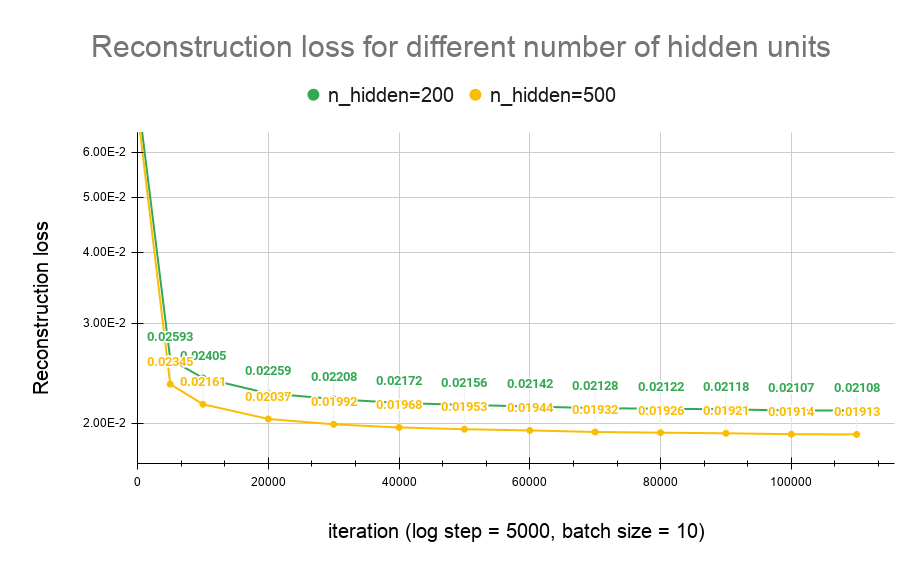
\includegraphics[width=1.\linewidth]{img/4.1 Reconstruction loss for different number of hidden units.png}
    \caption{Reconstruction loss for the two architectures, $784-500$ and $784-200$}
    \label{fig:rbm_recon_loss}
\end{figure}

In figure \ref{fig:rbm_sums} we can see the impact of a different number of nodes in the hidden layer on the reconstruction loss. More nodes allow for a better reconstruction.

\begin{figure}[H]
    \centering
    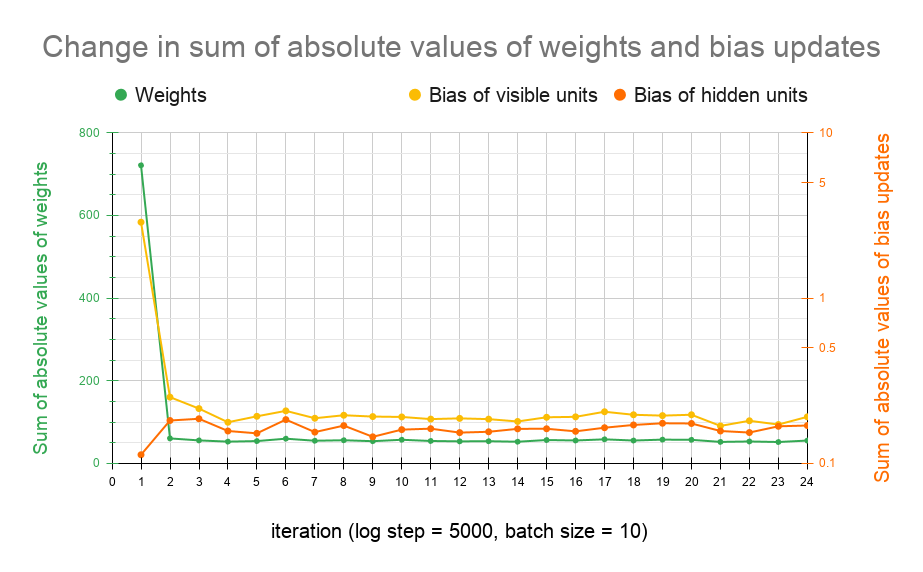
\includegraphics[width=1.\linewidth]{img/4.1 Change in sum of absolute values of weights and bias updates.png}
    \caption{Change in sum of absolute values of weights and biases for a RBM of 500 hidden nodes with momentum and no weight decay}
    \label{fig:rbm_sums}
\end{figure}

We and plotted receptive fields corresponding to the weights from a particular hidden node to the visible layer. We observed that some nodes have prominent parts that are specialized for the detection of curves and lines, as seen in the first row in figure \ref{fig:rmb_hnoi}. However, most of the receptive fields were hard to explain, like those in row 2 of figure \ref{fig:rmb_hnoi}. That is because all of the hidden nodes hold abstract and latent representations of the visible input, in this case forcefully compressed from 784 units into 500 and 200 units.

\begin{figure}[H]
    \centering
    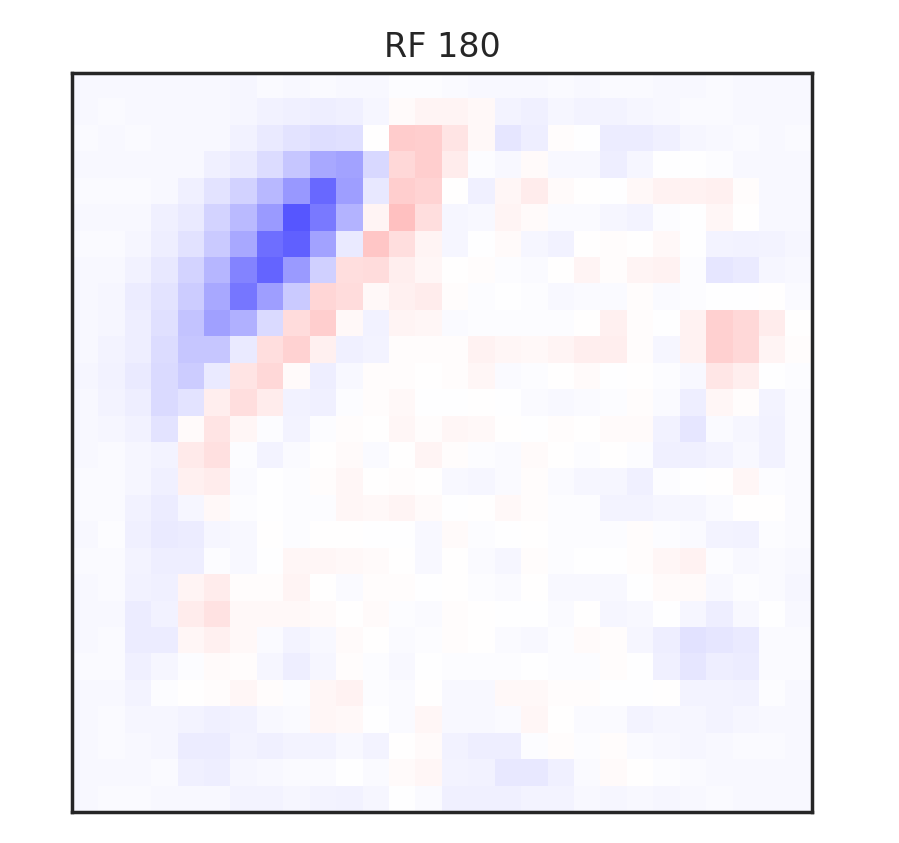
\includegraphics[width=0.21\linewidth]{img/rf_0180_2.png}
    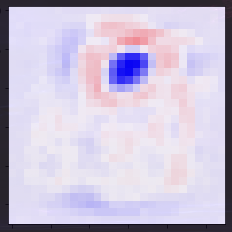
\includegraphics[width=.185\linewidth]{img/Hidden_node_of_interest.png}
    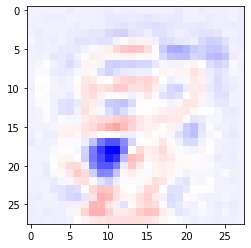
\includegraphics[width=.185\linewidth]{img/hnoi_02.png}
    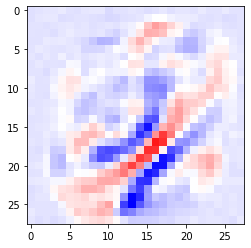
\includegraphics[width=.185\linewidth]{img/hnoi_03.png}
    \\
    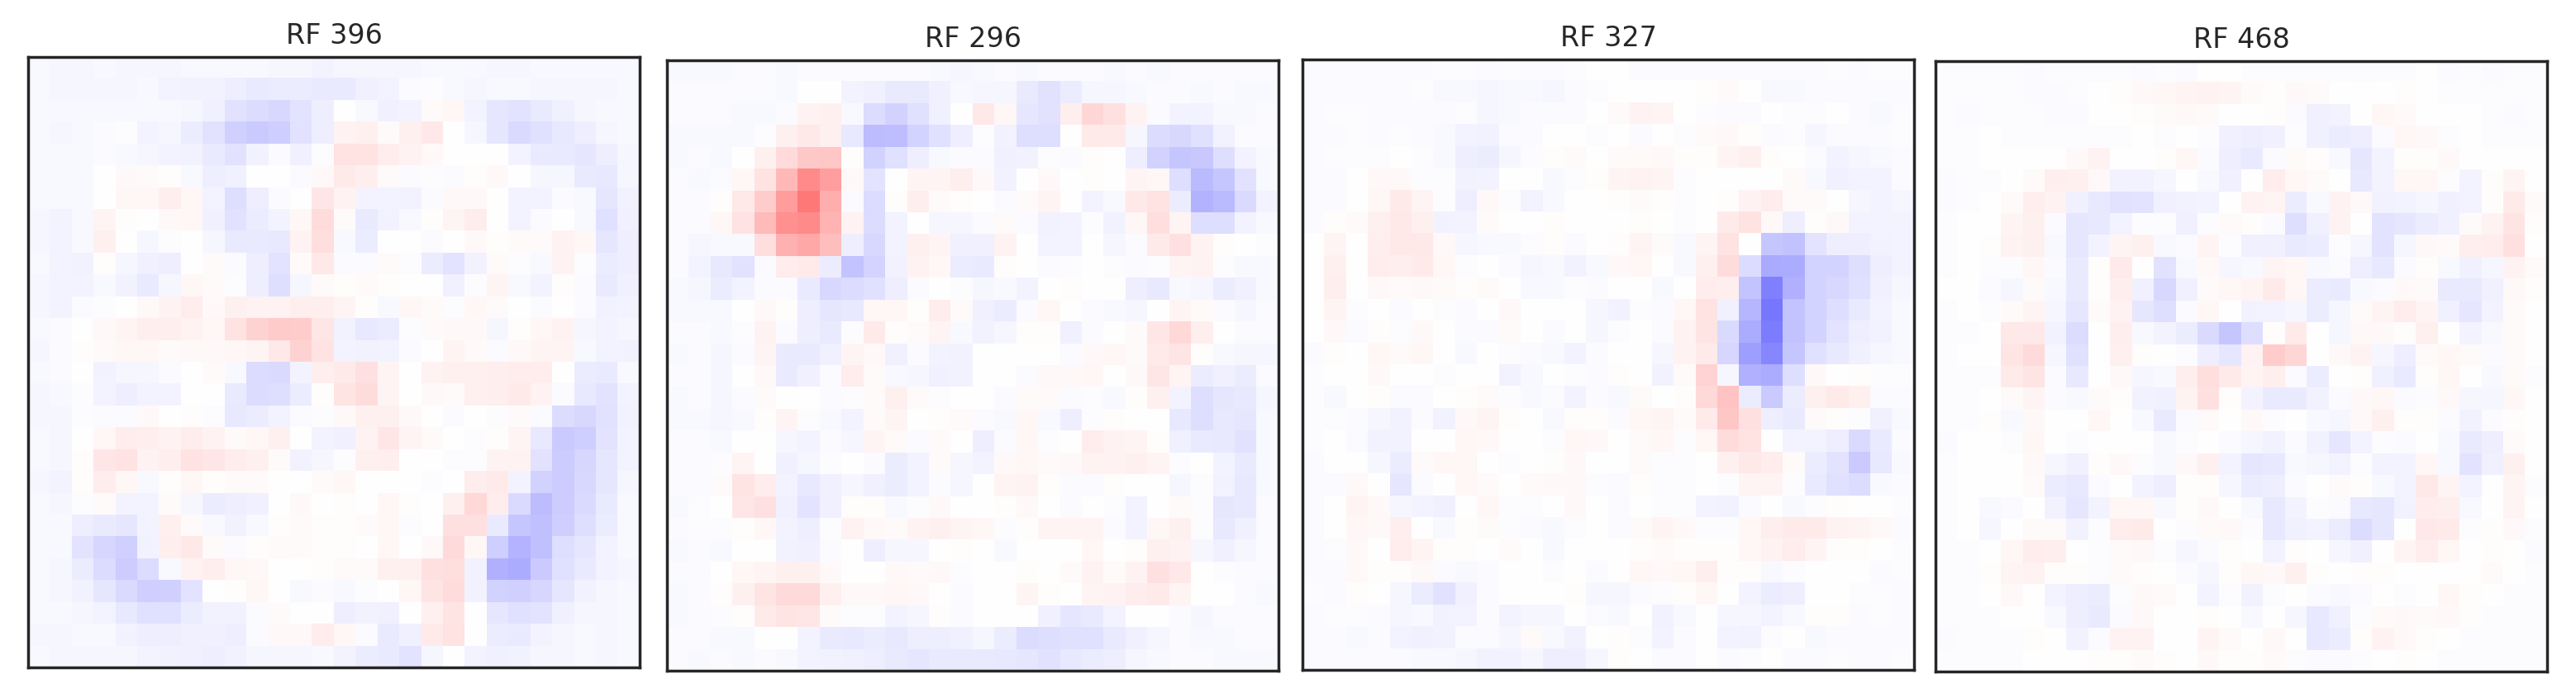
\includegraphics[width=.8\linewidth]{img/rfs.png}
    \caption{Receptive fields of a few hidden nodes of a $784-500$ RBM}
    \label{fig:rmb_hnoi}
\end{figure}


\subsection{Towards deep networks - greedy layer-wise pretraining}

For this part we turned our attention to a deep architecture called Deep Belief Networks (DBNs), essentially stacking RBMs together. We have implemented the greedy layer-wise pre-training, a method which uses unsupervised learning greedily, for each layer starting from the bottom, firstly using images, and then a trained layer's hidden representation as the visible units of the next layer RBM. 

Firstly we made a 3-layer stack of two RBMs (784-500-500 architecture) and observed their respective reconstruction losses. We noticed similar behaviour in reconstruction loss convergence, with topmost RBM having a slightly higher error than the RBM below (Figure \ref{fig:stacked_rbm_losses}).

\begin{figure}[H]
    \centering
    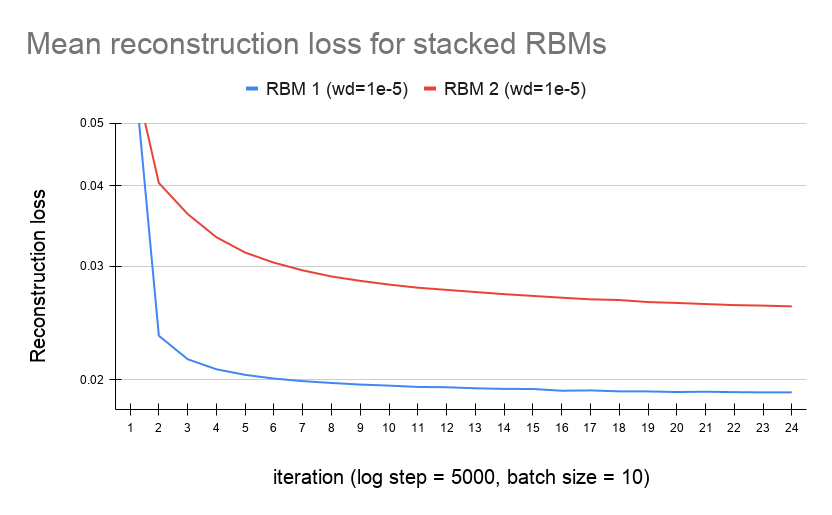
\includegraphics[width=.98\linewidth]{img/4.2 Mean reconstruction loss for stacked RBMs.png}
    \caption{Mean reconstruction loss for stacked RBMs}
    \label{fig:stacked_rbm_losses}
\end{figure}

Secondly, we added an additional RBM at the top of our previous network. The top RBM has 510 visible units (500 taken from the hidden layer of the RBM beneath it and 10 additional units used for digit labels) and 2000 hidden units. The top RBM is trained in the same way as the RBMs beneath with the exception of using training labels as our starting values of the 10 additional visible units. One-hot encoding is used for the conversion of a digit label to 10 units. This kind of network could now be considered a DBN and can be used for both image recognition and image generation purposes.

Observing the convergence and the recognition accuracy when classifying images, we can see the benefit of using around 15 Gibbs sampling iterations in the top layer in figure \ref{fig:accuracy_convergence}. In the network run shown in the figure, the accuracy achieved was 82.94\%, but during various runs, with changes in the under-the-hood network architecture details like when to use probabilities instead of samples during greedy pre-training and how to make the upward network pass during picture recognition, we managed to achieve recognition accuracy results reaching 94.5\% (Fig. \ref{fig:accuracy_convergence_probs}).

\begin{figure}[H]
    \centering
    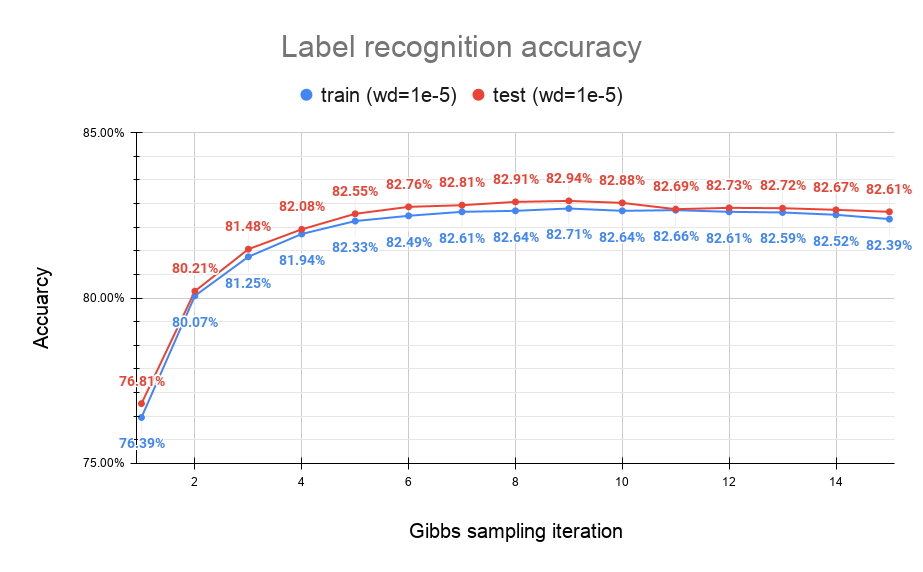
\includegraphics[width=.98\linewidth]{img/4.2 Label recognition accuracy(1).png}
    \caption{Label recognition accuracy}
    \label{fig:accuracy_convergence}
\end{figure}

\begin{figure}[H]
    \centering
    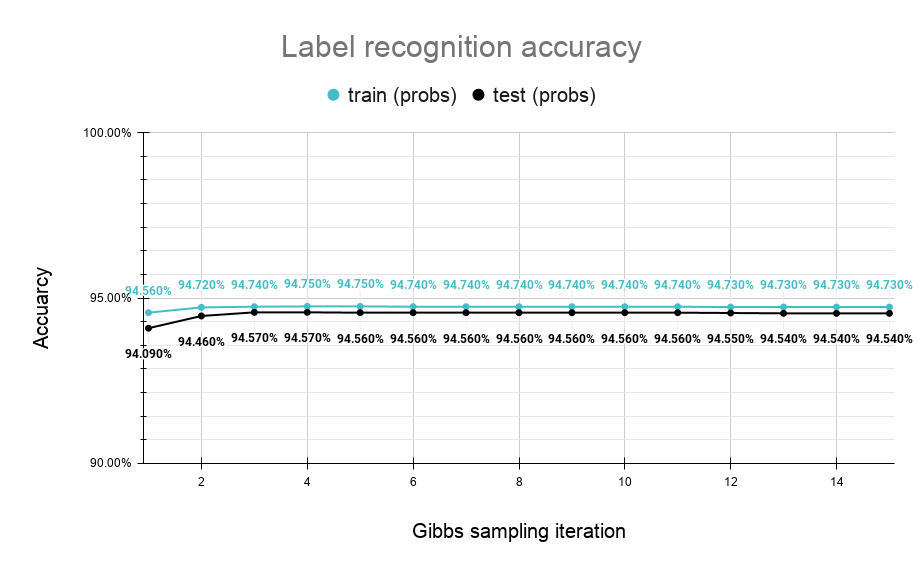
\includegraphics[width=.98\linewidth]{img/Label recognition accuracy (1).png}
    \caption{Label recognition accuracy is very high when passing probabilities from one RBM to the other and when using only probabilities during Gibbs sampling in topmost RBM for recognition classification. Having this modified network gave very bad results in picture generation}
    \label{fig:accuracy_convergence_probs}
\end{figure}

We also observed the behaviour of the probabilities in the 10 units responsible for digit classification in the visible layer of the topmost RBM. In figure \ref{fig:correct_and_incorrect_classification} we show two examples of correct digit classification and one example of an incorrect classification.

\begin{figure}
    \centering
    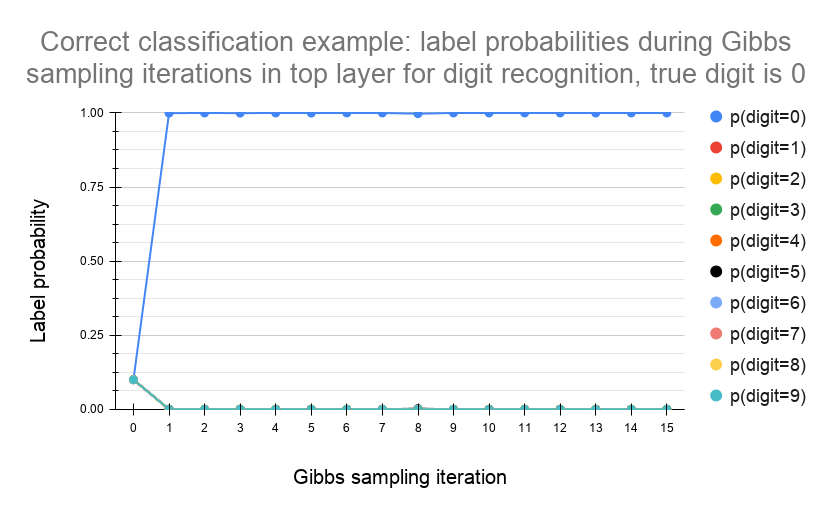
\includegraphics[width=.9\linewidth]{img/4.2 Correct classification example label probabilities during Gibbs sampling iterations in top layer for digit recognition, true digit is 0.png}
    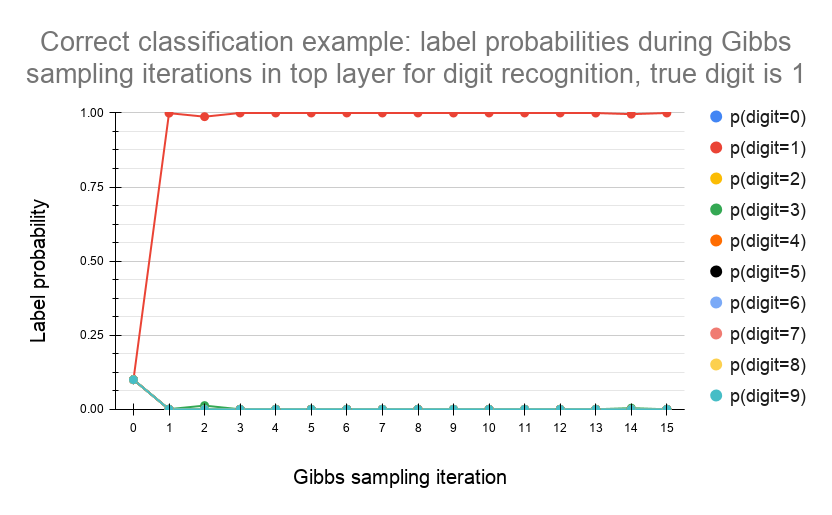
\includegraphics[width=.9\linewidth]{img/4.2 Correct classification example label probabilities during Gibbs sampling iterations in top layer for digit recognition, true digit is 1.png}
    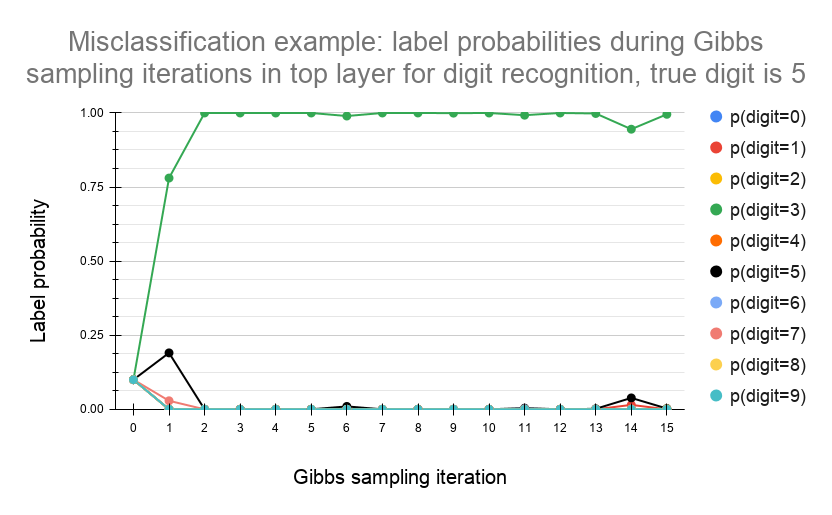
\includegraphics[width=.9\linewidth]{img/4.2 Misclassification example label probabilities during Gibbs sampling iterations in top layer for digit recognition, true digit is 5.png}
    \caption{Examples of correct classification in first two pictures and of incorrect classification in the last picture.}
    \label{fig:correct_and_incorrect_classification}
\end{figure}

Finally, we tested the generative abilities of our network. The network did not perform particularly well, but there were times when intuitive and expected patterns came up, such as those shown in Figure \ref{fig:digits}. These were the result of a couple of networks, trained with varying number of epochs, weight decay coefficients, and momentum coefficients. Better results could most certainly be acquired using supervised fine-tuning of the DBN.

\begin{figure}[H]
    \centering
    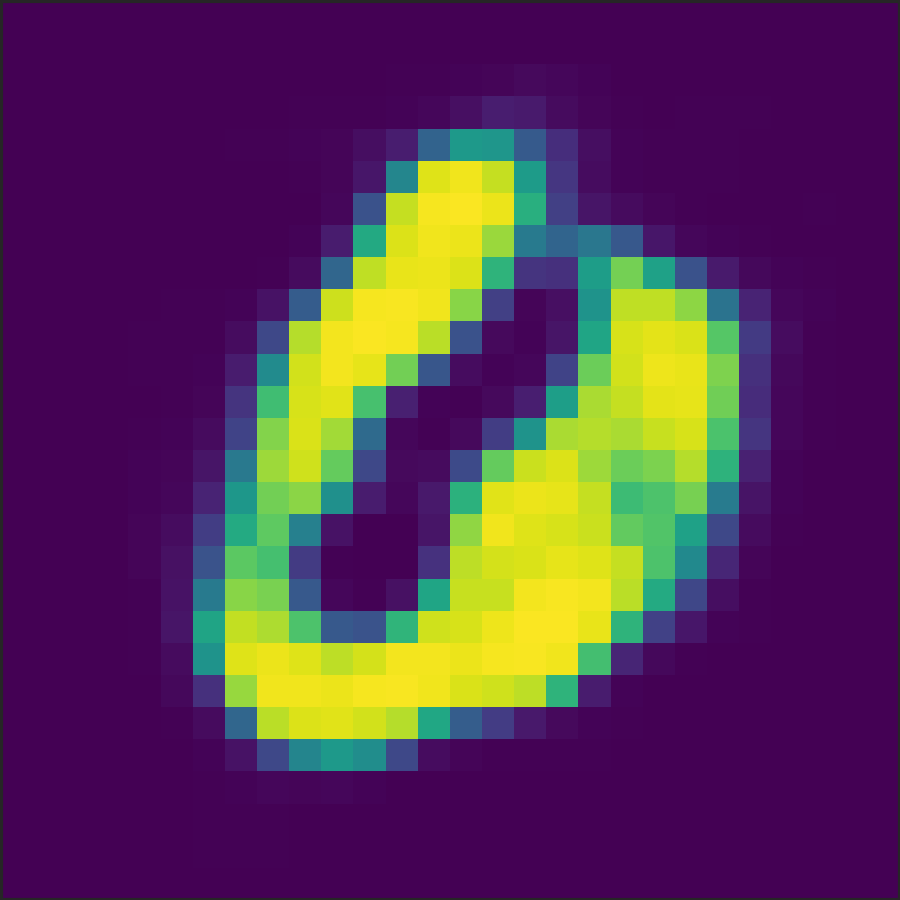
\includegraphics[width=.24\linewidth]{img/rbms.generate0 dbn_7_e=10.png}
    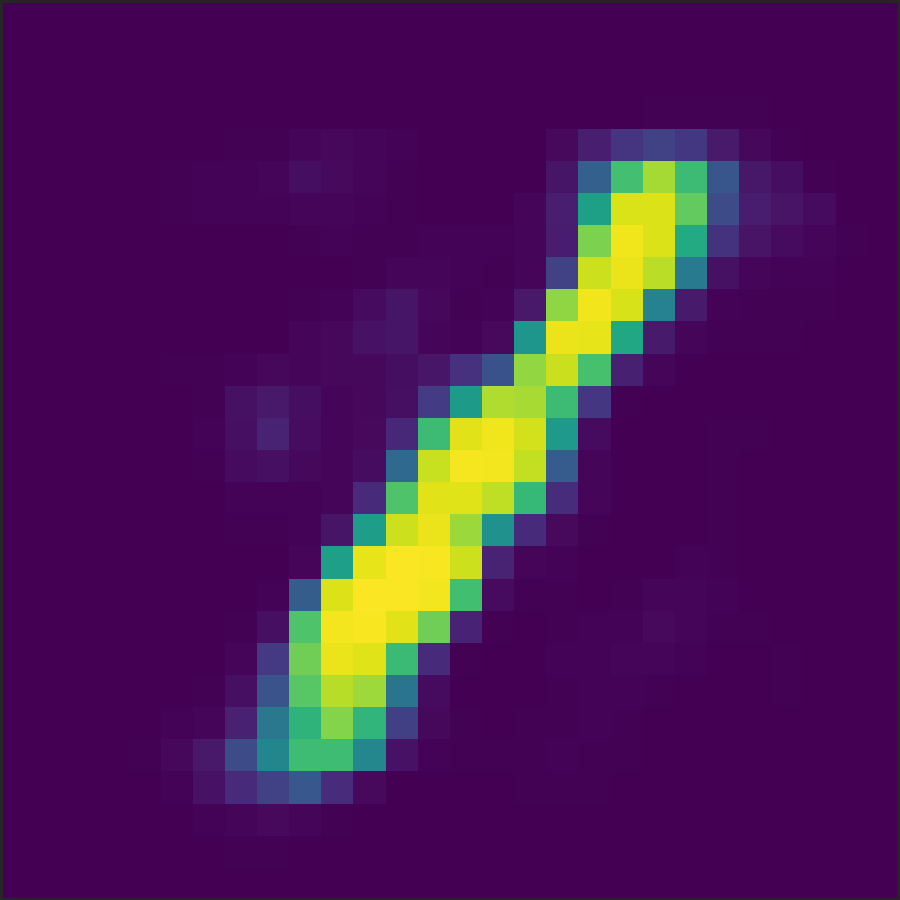
\includegraphics[width=.24\linewidth]{img/rbms.generate1 dbn_7_e=10.png}
    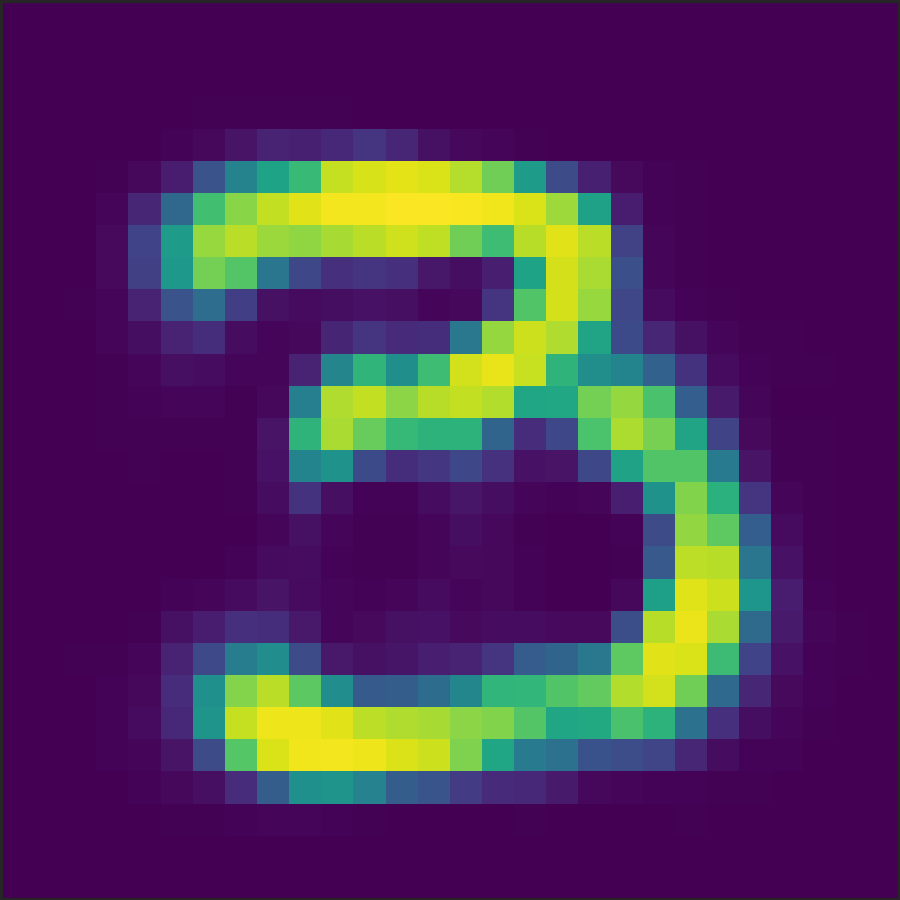
\includegraphics[width=.24\linewidth]{img/rbms.generate2 dbn_7_e=1.png}
    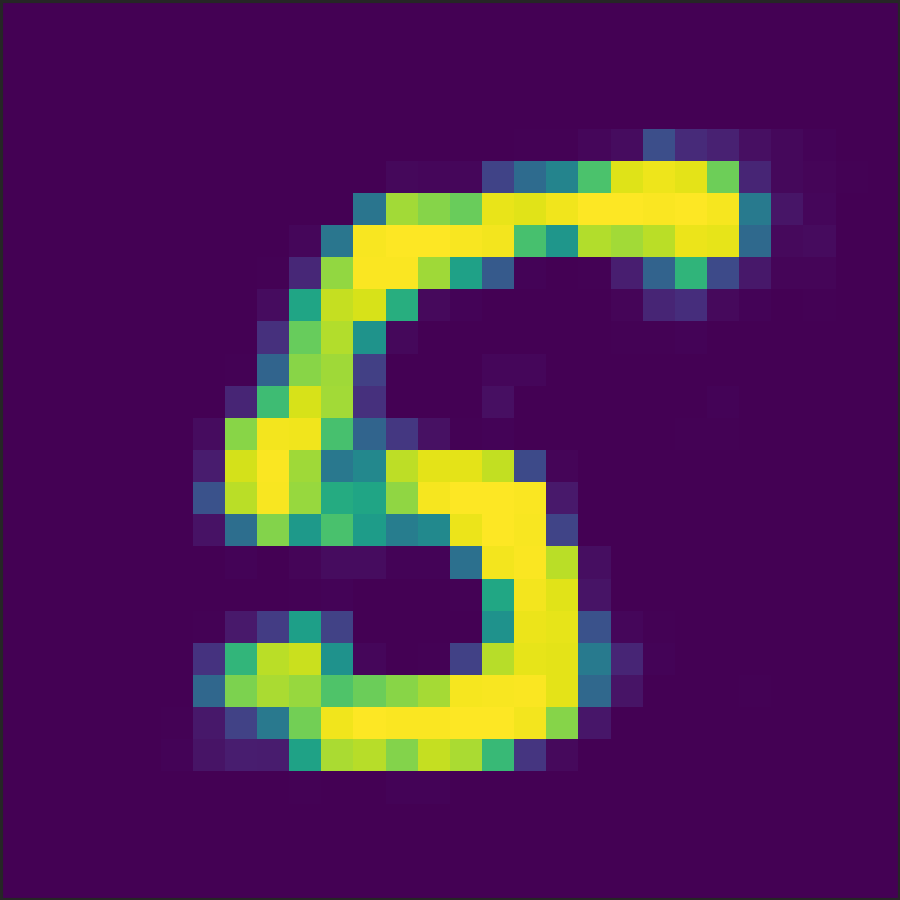
\includegraphics[width=.24\linewidth]{img/rbms.generate5 dbn_11_lr=0,01_wd=0,0e+00_m=0,7_b=10x_e=20.png}
    \caption{Mean reconstruction loss for stacked RBMs}
    \label{fig:digits}
\end{figure}

% \subsection{Supervised fine-tuning of the DBN}
%TD

\section{Final remarks}
The topic of the assignment was very interesting, but the instructions and materials could have been slightly clearer. It is easy to get lost in deciding when to use probabilities and when to use binary sampling; this could have been more clearly elaborated in terms of describing the intuition behind and letting the students know what exactly should they reproduce. This is important because the length of the training does not allow for many tests and it is hard to get intuition based on just a couple of tests. However, the exploratory part of the lab, even though perhaps too unguided, was interesting and advantageous in some learning aspects.
\end{document}
